\documentclass[conference]{IEEEtran} 
\IEEEoverridecommandlockouts 
\usepackage{cite} 
\usepackage{amsmath, amssymb, amsfonts} 
\usepackage{algorithmic} 
\usepackage{graphicx} 
\graphicspath{{./}{../docs/}{docs/}} 
\usepackage{textcomp} 
\usepackage{xcolor} 
\usepackage{booktabs} 
\usepackage{bm} 
\usepackage{url} 

\def\BibTeX{{\rm B\kern-.05em{\sc i\kern-.025em b}\kern-.08em 
       T\kern-.1667em\lower.7ex\hbox{E}\kern-.125emX}} 

\begin{document} 

\title{Route Diversity and Empirical Exploitability in Competitive Multi-Agent Reinforcement Learning with Dual-Archive Self-Play} 

\author {
\IEEEauthorblockN{Navadeep Nindra} 
\IEEEauthorblockA{\textit{Department of Mathematics} \\ 
\textit{SVNIT Surat}, India \\ 
u24mc006@amhd.svnit.ac.in} 
\and 
\IEEEauthorblockN{Brij Radadiya} 
\IEEEauthorblockA{\textit{Department of Mathematics} \\ 
\textit{SVNIT Surat}, India \\ 
u24mc005@amhd.svnit.ac.in} 
\and 
\IEEEauthorblockN{Shrey Marakana} 
\IEEEauthorblockA{\textit{Department of Mathematics} \\ 
\textit{SVNIT Surat}, India \\ 
u24mc009@amhd.svnit.ac.in} 
\and 
\IEEEauthorblockN{Shree Pastagia} 
\IEEEauthorblockA{\textit{Department of Mathematics} \\ 
\textit{SVNIT Surat}, India \\ 
u24mc011@amhd.svnit.ac.in} 
} 

\maketitle 

\begin{abstract} 
Self play allows learning agents to play against each other, but the fact that the agent's opponent is constantly changing can mean that previously good and effective routes become less common. We look at this in the Three Bridges Arena where an Attacker crosses one of three bridges and a Defender tries to intercept it. We compare direct self play with Dual Archive training which also uses saved opponent policies. In 150 matched reviews against an unresponsive Defender, direct self play used the North bridge 46.0\% of the time and the South 16.1\%, with 17.3\% timeouts. Dual Archive used the routes more uniformly (1.567 bits of entropy, 98.9\% of the three route maximum) and had no timeouts at all. Against six of the tested defenders its worst case security score was -0.187 versus -0.207 and its measured exploitability was 0.140 versus 0.160. The pooled win rate difference was not statistically significant. In a separate 500 episode configurable arena benchmark the three target Attacker beat its learned Defender 97.6\% of the time and beat Greedy Pursuit 28.2\% of the time. Route application is just an indirect measure; these experiments don't actually test for devastating forgetting. 
\end{abstract} 

\begin{IEEEkeywords} 
Multi-Agent Reinforcement Learning, Self-Play, Route Diversity, Exploitability, Potential-Based Reward Shaping, Zero-Sum Games. 
\end{IEEEkeywords} 

\section{Introduction} 
In multi-agent reinforcement learning (MARL) you've got a number of different, diverse decision makers operating in a single shared environment. In the case of self play the agents learn by playing against each other and as each agent is constantly changing so is its opponent. 

This makes the learning non-stationary. In some games you can have cycles of strategy: one strategy is countered by another, which in turn is countered. Cliff and Miller used the Red Queen analogy to describe analogous phenomena in co-evolution \cite{cliff1995tracking}. We use it purely as an analogy; our grid game is not a model of life at all. 

A related issue is whether an agent ceases to use a route it previously used. We measure bridge choice as an indirect indicator of route variety; a change in the frequency of route use doesn't necessarily mean that the agent has lost the ability to use that route. 

We look at these queries in the Three Bridges Arena, a two player grid game. The Attacker is trying to cross the river and get to the target and the Defender is trying to catch it. There are four blocked cells which leaves three possible crossings: North, Centre and South. A single Defender cannot guard all three of those at once so the Attacker will always have more than one route. 

This paper describes the arena, archive-training method, and evaluation: 
\begin{enumerate} 
       \item \textbf{Game and training method :} We define the arena, zero-sum rewards, potential shaping and PPO-based Dual Archive training. 
       \item \textbf{Evaluation measures :} We measure route usage via Shannon entropy and opponent robustness via the security and exploitability values over a corrected defender pool. 
       \item \textbf{Results :} The archive-trained policy used more routes and showed improved worst-case robustness in the reported evaluations.
\end{enumerate}
\section{Related Work}

\subsection{Self-Play and Policy Cycling in MARL}
When both policies are adjusting during training then each agent is up against a moving target. Cliff and Miller described exactly the same kind of cycling that occurs in co-evolution as a Red Queen dynamic \cite{cliff1995tracking}. Our work is then to ask whether the inclusion of saved opponents has any effect on route application and performance in this scenario.

\subsection{Memory Reservoirs, Double Oracle, and PSRO}
Population based methods keep the prior policies on hand as opponents. Our dual archive approach uses a small, symmetric reservoir of frozen snapshots for both players, with the majority of the archive still being devoted to most recent self play. The training schedule is described in Section IV.

\subsection{Potential-Based Reward Shaping in Zero-Sum Games}
Sparse rewards make navigation very difficult to learn. Ng et al. \cite{ng1999policy} demonstrate that under the conditions they describe, a potential difference term $F(s,s') = \gamma\Phi(s') - \Phi(s)$ will maintain both perfect and optimal policies. In our game we apply equal and opposite shaping rewards so as to preserve the zero-sum reward structure. We assess the resulting policies empirically rather than state a new equilibrium preservation result.

\section{Game Formulation and Theoretical Framework}

\subsection{Two-Player Zero-Sum Markov Game}
We model the interaction as a discrete-time, two-player zero-sum Markov game:
\begin{equation}
\mathcal{M} =\langle \mathcal{S}, \mathcal{A}_1, \mathcal{A}_2, \mathcal{P}, \mathcal{R}_1, \mathcal{R}_2, \gamma \rangle
\end{equation}
where:
\begin{itemize}
       \item $\mathcal{S}$ is a subset of $[0,1]^6$ and represents the normalised observation space (i.e. the coordinates of both agents and the target).
       \item $\mathcal{A}_1$, $\mathcal{A}_2$ are the discrete action sets of the attacker (Player 1) and defender (Player 2) respectively, each with $|\mathcal{A}_i| = 5$.
       \item $\mathcal{P}: \mathcal{S} \times \mathcal{A}_1 \times \mathcal{A}_2 \longrightarrow \mathcal{S}$ is the deterministic state transition function.
       \item $\mathcal{R}_1$, $\mathcal{R}_2: \mathcal{S} \times \mathcal{A}_1 \times \mathcal{A}_2 \to \mathbb{R}$ are the reward functions with $\mathcal{R}_1(s,a_1,a_2) + \mathcal{R}_2(s,a_1,a_2) = 0$ for all $s,a_1,a_2$.
       \item $\gamma$ is in the range $[0,1)$, set to $\gamma = 0.99$.
\end{itemize}

\subsection{The Three Bridges Arena}
The game is played on a grid of width $W=11$ ($X \in \{0,\dots,10\}$) and height $H=7$ ($Y \in \{0,\dots,6\}$). There's a river running down column $X=5$ which splits the arena in two. Fig.~\ref{fig:arena} shows the crossings and target side:
\begin{itemize}
       \item \textbf{Attacker side ($X \in [0, 4]$) :} The Attacker spawns at a uniformly random location with $X_A \in [0, 3]$ and $Y_A \in [0, 6]$.
       \item \textbf{River ($X =5 $):} Four blocked cells at $(5, 0), (5, 2), (5, 4), (5, 6)$ leave three open bridges:
       \begin{align}
       \text{North Bridge :} \quad & b_N =( 5, 1) \\
       \text{Center Bridge :} \quad & b_C =( 5, 3) \\
       \text{South Bridge :} \quad & b_S =( 5, 5)
       \end{align}
       \item \textbf{Defender side ($X \in [6, 10]$) :} The Defender spawns uniformly with $X_D \in [6,9]$ and $Y_D \in [0,6]$ (excluding the Citadel cell).
       \item \textbf{Citadel :} A fixed target at $(X_T,Y_T)=(10,3)$
\end{itemize}
\begin{figure}[t]
\centering
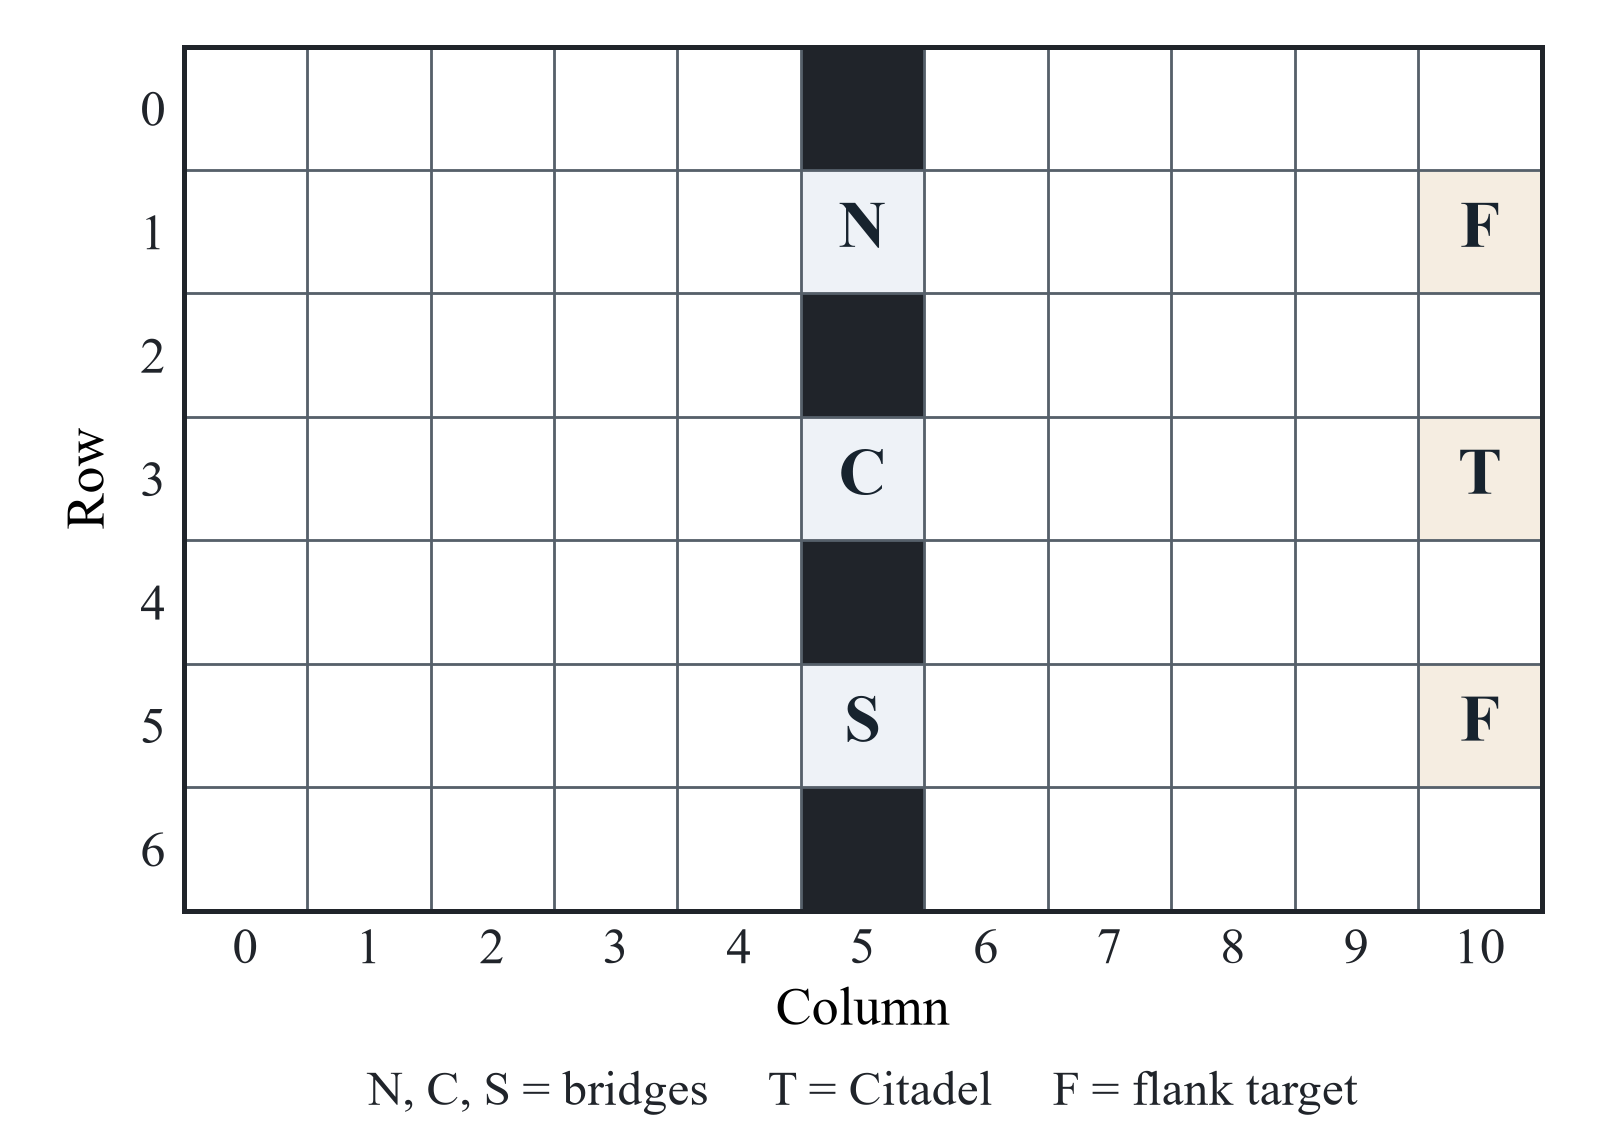
\includegraphics[width=\columnwidth]{paper_figures/three-bridges-arena.png}
\caption{Arena layout. N, C and S denote the open bridges over the river; the dark cells are blocked. Targets vary from layout to layout: the Citadel is in the centre, with the various layouts activating different cells along the eastern edge.}
\label{fig:arena}
\end{figure}

\subsection{State and Actions}

The state is the pair of agent positions and the target position, normalized by $(W-1)$ and $(H-1)$:

\begin{equation}
s_t = \left[ \frac{x_A}{10}, \frac{y_A}{6}, \frac{x_D}{10}, \frac{y_D}{6}, \frac{x_T}{10}, \frac{y_T}{6} \right]^T
\end{equation}

This normalization means that $s_t \in [0, 1]^6$ which aids in stabilizing the training of the value network.

At each step, both agents act simultaneously and choose from the set of actions $\mathcal{A} = \{\text{UP}, \text{DOWN}, \text{LEFT}, \text{RIGHT}, \text{STAY}\}$. Agent positions are updated using the following equations:

\begin{equation}
\bm{p}_{i, t+1} = \bm{p}_{i, t} + \bm{v}(a_{i, t})
\end{equation}

The bounds of the grid are $0 \leq x < 11$, $0 \leq y < 7$ and there are blocked cells at the positions $(5, 0)$, $(5, 2)$, $(5, 4)$ and $(5, 6)$. If an agent attempts to move into a blocked cell or a wall, the position of the agent doesn't change ($ \bm{p}_{i, t+1} = \bm{p}_{i, t} $).

\subsection{Terminal Conditions and Priority}

An episode ends when any of the conditions listed below occur:

1. The Attacker enters the Citadel (reaches cell $(10, 3)$): Payoffs: $R_A = +10, R_D = -10$

2. The Defender captures the Attacker before it reaches the Citadel: Payoffs: $R_A = -10, R_D = +10$

3. Timeout: If $T_{\max} = 75$ steps are taken and neither of the conditions 1 or 2 occur: Payoffs: $R_A = R_D = 0$.

In the case that the conditions 1 and 2 occur at the same time, priority is given to condition 1 (capture is ignored if Citadel is reached).

This removes any possible ambiguity as to who wins.

A simple example of mixed route choices using the 3-route matching model is given. The payoff matrix and outcome of this simplified model are in Appendix~\ref{app:matching}. The result only applies to the simplified model and not to all states and moves in the full grid game.

\subsection{Zero-Sum Discounted Potential-Based Reward Shaping}

For terminal rewards to be sparse by $\pm 10$ over a horizon of 75 steps exploration is going to be very slow and noisy. We therefore use potential based shaping.

The Attacker's distance-to-target potential $D_A(x,y)$ is defined as follows, based on which side of the river he/she is on:

\begin{equation}
D_A(x,y) =
\begin{cases}
\displaystyle\min_{b_y \in \{1,3,5\}}
\left(\begin{aligned}
&\lvert x - 4\rvert + \lvert y - b_y\rvert\\
&\quad + 6 + \lvert b_y - 3\rvert
\end{aligned}\right), & x \le 4, \\
\lvert x - 10\rvert + \lvert y - 3\rvert, & x > 4.
\end{cases}
\end{equation}

For state $s$ we write $D_A(s_A)$ for $D_A(x_A,y_A)$ where $s_A$ denotes the position of the attacker.

The quantity \(\lvert b_y-3\rvert\) is the vertical distance from a bridge exit to the citadel row, \(y=3\). Thus, all three routes have the same remaining vertical distance. With \(\gamma=0.99\), the shaping term for progress toward the target is:

\begin{equation}\label{eq:shaping_tgt}
F_{\text{tgt}}(s,s') = \alpha_{\text{tgt}} \left[ D_A(s_A) - \gamma D_A(s'_A) \right]
\end{equation}

with $\alpha_{\text{tgt}} = 0.3$.

To balance the pursuit and evasion we added a relative potential $D_{\text{rel}}(s) = |x_A - x_D| + |y_A - y_D|$ with $\alpha_{\text{rel}} = 0.2$.

\begin{equation}
F_{\text{rel}}(s, s') = \alpha_{\text{rel}} \left[ D_{\text{rel}}(s) - \gamma D_{\text{rel}}(s') \right]
\label{eq:shaping_rel}
\end{equation}

 Shaping rewards for a pair of players are defined symmetrically:

\begin{align}
F_A(s, s') &= +F_{\text{tgt}}(s, s') - F_{\text{rel}}(s, s') \\
F_D(s, s') &= -F_{\text{tgt}}(s, s') + F_{\text{rel}}(s, s')
\end{align}

Because of the definition of shaping, for each transition, it holds that $F_A(s,s') + F_D(s,s') = 0$. Therefore, the total rewards for player A and player D are opposites for each other, and both are zero:

\begin{equation}
R_A(s, a_1, a_2) + R_D(s, a_1, a_2) = 0 \quad \forall s, s' \in \mathcal{S}
\end{equation}

Rewarding shaping, or in other words, negative rewarding in shaping, is in fact a zero-sum game, since, in this case, there is neither a reward gain nor punishment. The experiments test the effect of negative rewarding shaping on the learned policies. They do not provide any evidence as to whether negative rewarding shaping maintains the equilibrium set of the complete game.

\begin{figure}[h]

\centering
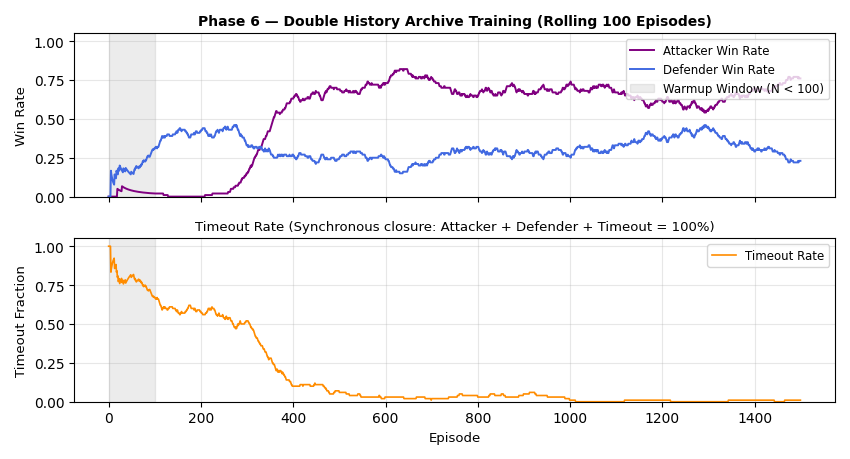
\includegraphics[width=0.9\columnwidth]{phase6_archive_curve.png}

\caption{Dual-Archive - Training was done with over 1,500 episodes. The figures at the top are the rolling win rates of the Attacker (purple) and Defender (blue): Here the Defender's win rate is rolling at about 33\% while the Attacker's is rolling at 65\% and is consistent with the structural edge that Attackers have with three bridges over the Defender. The time out rate is at about 80\% in the early exploration phase and drops to less than 2\% when all objects are converged.}

\label{fig:training_curve}

\end{figure}

\section{Dual-Archive Co-Evolutionary Framework}

\subsection{Why plain self-play is fragile}

In our work we state that the three trained models are named as follows: Phase 3 has a fixed-opponent model, Phase 4 is direct self-play, and Phase 6 is Dual-Archive.

For direct self-play (Phase 4), the parameter $\theta_A$ is updated using parameter $\theta_D$:

 \begin{align}
\theta_{A, k+1} & \leftarrow \theta_{A, k} + \eta_A \nabla_{\theta_A} \mathcal{J}_A(\theta_{A, k}, \theta_{D, k}) \\
\theta_{D, k+1} & \leftarrow \theta_{D, k} + \eta_D \nabla_{\theta_D} \mathcal{J}_D(\theta_{A, k}, \theta_{D, k})
\end{align}

  Both updated policies no longer have a fixed opponent since both are happening at the same time. In this case, as the Attacker learns how to break through the North bridge, the Defender learns to block the North bridge. The Attacker then take his/her turn to the South bridge and can end practicing North or Center. This can result in overloading cycling and to "burst" onto a couple of routes.

\subsection{Dual-Archive Architecture}
This is based on a symmetric Dual-Archive method (Phase 6) to anchor learning without a large league training system. We have two banks of legacy policies, which we will denote $\mathcal{H}_A$ and $\mathcal{H}_D$ for Attacker and Defender respectively. These are defined as follows:

\begin{equation}
\begin{split}
\mathcal{H}_A = \{\pi_A^{(1)}, \pi_A^{(2)}, \dots, \pi_A^{(K)}\} \\
\mathcal{H}_D = \{\pi_D^{(1)}, \pi_D^{(2)}, \dots, \pi_D^{(K)}\}
\end{split}
\end{equation}

There is a 300-episode warm up period after which a frozen copy of the policies is taken every $E_{\text{snap}} = 100$ episodes.

During training episodes, one of the three opponent configurations listed below is employed.

\begin{itemize}

\item Active co-evolution (60\%): Both Attacker and Defender update their policies.

\item Attacker against history (20\%): The active Attacker takes one of history Defender snapshots, chosen from the uniform distribution, $\pi_D \sim \mathcal{U}(\mathcal{H}_D)$. Only the Attacker's policy is updated.

\item Defender against history (20\%): The active Defender takes on an Attacker who is modeled with a snapshot from some randomly chosen $\pi_A \sim \mathcal{U}(\mathcal{H}_A)$. Only the Defender's policy is updated.

\end{itemize}

The 60\% share has agents learning from the most recent opponents, while the 20\% shares employ agents learning older opponent behaviors to reduce forgetting.
\subsection{Actor-Critic PPO Implementation}
Both agents learn using Proximal Policy Optimization (PPO) \cite{schulman2017proximal}. Two fully connected layers each containing 64 units and with a tanhs activation functions are used for the actor $\pi_\theta(a \mid s)$ and the critic $V_\phi(s)$.

The policy is optimized using the cropped surrogate loss function
\begin{equation}
\mathcal{L}^{\text{CLIP}}(\theta) = \hat{\mathbb{E}}_t \left[ \min\left( r_t(\theta)\hat{A}_t, \, \text{clip}(r_t(\theta), 1-\epsilon, 1+\epsilon)\hat{A}_t \right) \right]
\end{equation}
where $r_t(\theta) = \frac{\pi_\theta(a_t \mid s_t)}{\pi_{\theta_{\text{old}}}(a_t \mid s_t)}$ and the clipping threshold is $\epsilon = 0.20$. Advantaged are calculated in a Monte Carlo manner, $\hat{A}_t = G_t - V_\phi(s_t)$, and then are “normalized” within each batch of generations. The actions which fall in blocked cells are shaded out.

4 epochs $\times$ 64 mini-batches every epoch, for each update, with updates being made every 20 episodes (every 10 for the Phase 3 baseline). The total loss is
\begin{equation}
\mathcal{L}_{\text{total}}(\theta, \phi) = -\mathcal{L}^{\text{CLIP}}(\theta) + 0.5 \, \mathcal{L}^{\text{VF}}(\phi) - 0.01 \, \mathcal{S}[\pi_\theta](s_t)
\end{equation}
with learning rates $\alpha_{\text{actor}} = 10^{-3}$ and $\alpha_{\text{critic}} = 2 \times 10^{-3}$, and gradient-norm clipping at $\tau_{\text{clip}} = 0.5$.

\begin{figure*}[t]
\centering
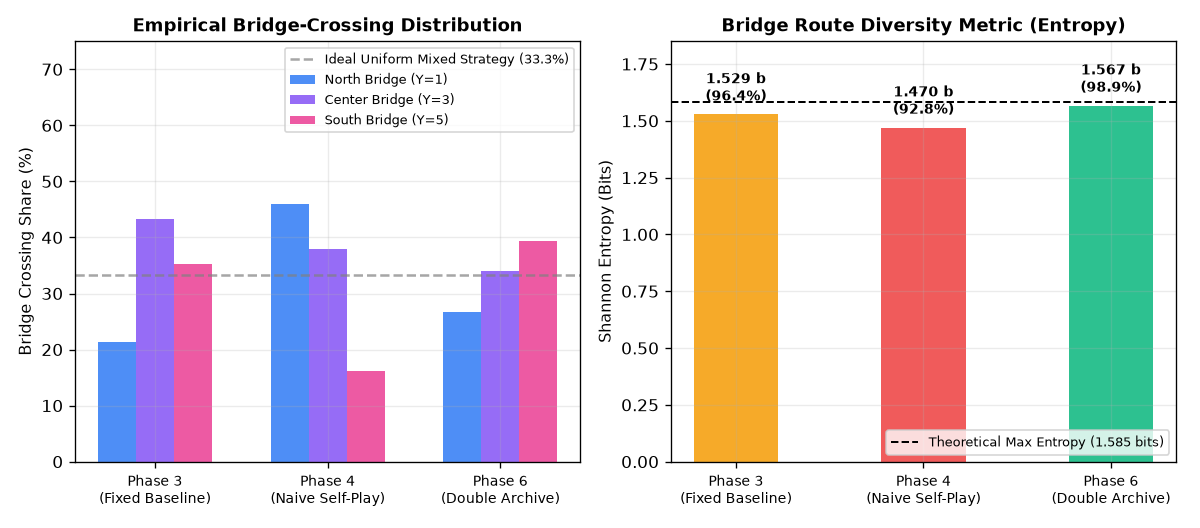
\includegraphics[width=0.90\textwidth]{bridge_diversity_chart.png}
\caption{Diversity over 150 paired evaluation seeds for bridge-routes. Left: y share of crosses in the North ($Y=1$) and Center ($Y=3$) bridges and South ($Y=5$) bridge compared to a uniform 33.3\%. Right: Routing entropy of Shannon. The Dual-Archive co-evolution (Phase 6) achieves 1.567 bits (98.9\% of the maximum) and an uneven route distribution, but Direct self-play (Phase 4) shows 17.3\% timeouts.}
\label{fig:bridge_diversity}
\end{figure*}

\section{Evaluation Methodology}

Two evaluation protocols comparing route use and exploitability are used.

A variant on route diversity is using Shannon entropy.
Over 150 pairs of evaluation seeds we record successful river crossings at $X=5$. Defender is passive and does not move around, Attacker's route choice is measured in the absence of being actively intercepted. If at any point the Attacker does not have $X \ge 6$ the crossing doesn't count. This only depicts those routes that the policy uses instead of demonstrating if the policy wants to use another route that it does not use often.

Using the notation above, let $C_b$ represent the number of successful crossings across bridge $b \in \{b_N, b_C, b_S\}$. The percentage of traffic crossing each bridge is
\begin{equation}
p_b = \frac{C_b}{\sum_{k \in \{N, C, S\}} C_k}
\end{equation}
and the Shannon route entropy is
\begin{equation}
H(\text{Routes}) = -\sum_{b \in \{N, C, S\}} p_b \log_2(p_b)
\end{equation}
Its bounds are
\begin{align}
H_{\max} &= \log_2(3) \approx 1.585 \text{ bits}\;(\text{uniform, 33.3\% per route}) \\
H_{\min} &= 0 \text{ bits} \text{ (all crossings are on one bridge)}
\end{align}
The diversity ratio is $\rho_{\text{div}} = \frac{H(\text{Routes})}{H_{\max}} \times 100\%$. A timeout is a period of time where the Attacker is not crossed in 75 steps.

\subsection{Empirical Game-Theoretic Analysis (EGTA)}
A game-theoretic approach, which does not rely exclusively on win rates, but is empirical, is used to judge the distance between the policy and a minimax solution. Construct a set of defenders, $\mathcal{P}_{\text{def}}$:
\begin{enumerate}
    \item \textbf{North Camper ($Y=1$):} A Static camper parked at the North bridge.
    \item \textbf{Center Camper ($Y=3$):} An unchanging camper at the Center bridge.
    \item \textbf{South Camper ($Y=5$)} is a stationary camper located at the South bridge.
    \item A defender that moves back and forth on the east bank of the river between $Y=1$ and $Y=5$ is called a River Patroller.
    \item Trained policies: $\pi_{D, \text{Phase 4}}$ and $\pi_{D, \text{Phase 6}}$.
\end{enumerate}

The empirical payoff matrix $\bm{M} \in \mathbb{R}^{m \times n}$ holds the Attacker's net win margin of Attacker policy $i$ against defender $j$:
\begin{equation}
M_{i, j} = \text{WinRate}(\pi_i, d_j) - \text{CatchRate}(\pi_i, d_j) \in [-1.0, +1.0]
\end{equation}
From $\bm{M}$ we compute:
\begin{enumerate}
    \item \textbf{Minimax game value ($v^*$):} Found with 50,000 iterations of zero-sum Fictitious Play on the empirical meta-game, giving $v^* = -0.046$.
    \item \textbf{Security level ($v_{\text{sec}}$):} The worst net margin of policy $\pi_i$ against any defender in the suite:
    \begin{equation}
    v_{\text{sec}}(\pi_i) = \min_{j \in \mathcal{P}_{\text{def}}} M_{i, j}
    \end{equation}
    \item \textbf{Empirical exploitability ($\delta_{\text{meta}}$):} The gap between the game value and the security level:
    \begin{equation}
    \delta_{\text{meta}}(\pi_i) = v^* - v_{\text{sec}}(\pi_i)
    \end{equation}
\end{enumerate}
A lower $\delta_{\text{meta}}$ means the policy is closer to the minimax value within the set of strategies we tested.

\section{Results and Discussion}

\begin{table*}[t]
\caption{Bridge Crossing Distribution and Route Diversity ($N=150$ Paired Evaluation Seeds)}
\label{tab:bridge_diversity}
\centering
\resizebox{\textwidth}{!}{%
\begin{tabular}{lccccccc}
\toprule
\textbf{Model} & \textbf{North ($Y=1$)} & \textbf{Center ($Y=3$)} & \textbf{South ($Y=5$)} & \textbf{Timeouts} & \textbf{Entropy ($H$)} & \textbf{Diversity \%} & \textbf{Profile} \\
\midrule
Phase 3 (Fixed Baseline)        & 21.3\% & 43.3\% & 35.3\% & 0.0\%  & 1.529 bits & 96.4\% & Baseline navigation \\
Phase 4 (Direct Self-Play)      & 46.0\% & 37.9\% & 16.1\% & 17.3\% & 1.470 bits & 92.8\% & North-heavy, 17.3\% timeouts \\
\textbf{Phase 6 (Dual Archive)} & \textbf{26.7\%} & \textbf{34.0\%} & \textbf{39.3\%} & \textbf{0.0\%}  & \textbf{1.567 bits} & \textbf{98.9\%} & \textbf{Balanced use of all three bridges} \\
\bottomrule
\end{tabular}%
}
\end{table*}

\begin{table*}[t]
\caption{Meta-Game Security Levels and Exploitability ($N=150$ Paired Evaluation Seeds)}
\label{tab:exploitability}
\centering
\begin{tabular}{lccccc}
\toprule
\textbf{Attacker Policy} & \textbf{Security Level ($v_{\text{sec}}$)} & \textbf{Worst-Case Win Rate} & \textbf{Exploitability ($\delta$)} & \textbf{Average Win Margin} & \textbf{Patroller Win Rate} \\
\midrule
Phase 4 (Direct Self-Play)      & -0.207 & 39.3\% & 0.160 & +0.190 & 76.0\% \\
\textbf{Phase 6 (Dual Archive)} & \textbf{-0.187} & \textbf{31.3\%} & \textbf{0.140} & \textbf{+0.184} & \textbf{81.3\%} \\
\bottomrule
\end{tabular}
\end{table*}

\subsection{Route Use Under Archive Training}
Table~\ref{tab:bridge_diversity} and Fig.~\ref{fig:bridge_diversity} show the crossing distributions.

The direct self-play agent (Phase 4) favors one side. It sends 46.0\% of its crossings through the North bridge and only 16.1\% through the South bridge, and its entropy is 1.470 bits (92.8\% of the maximum). It also times out in 17.3\% of episodes even though the river is undefended. A likely explanation is that when the spawn point makes the North bridge hard to reach, the policy does not redirect to the southern bridges and runs out of time. We have not tested this explanation directly.

The Dual-Archive policy (Phase 6) spreads its crossings over all three bridges: 26.7\% North, 34.0\% Center, and 39.3\% South. Its entropy is \textbf{1.567 bits}, or \textbf{98.9\% of the maximum} (1.585 bits), and it has \textbf{no timeouts}. A plausible reason is that it trained against archived defenders that had guarded different bridges, so it kept using several routes. Our measurements show this pattern but do not prove the cause.

\begin{figure*}[!t]
\centering
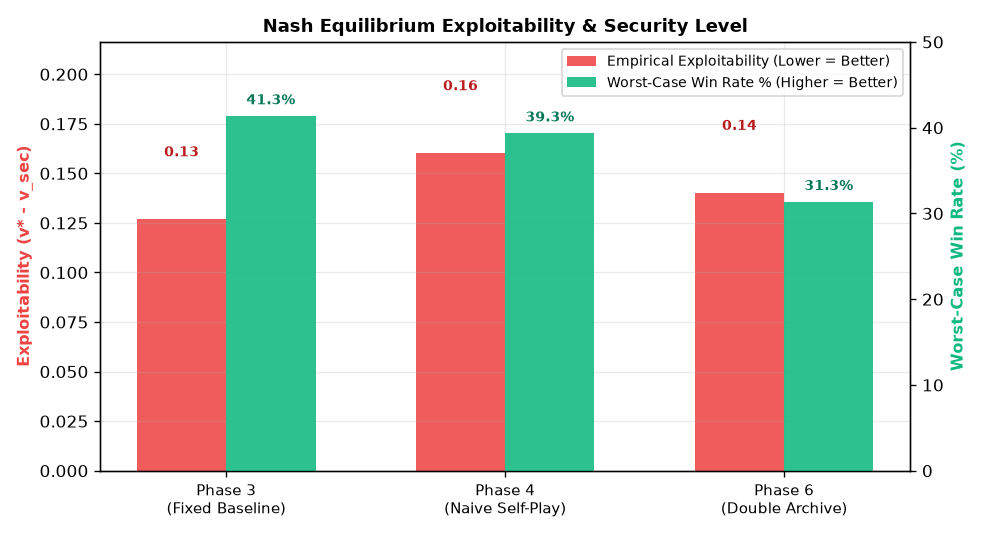
\includegraphics[width=0.78\textwidth]{nash_exploitability_chart.png}
\caption{Empirical exploitability ($\delta$) and worst-case win rate against the tested defender types. Dual-Archive co-evolution lowers exploitability from 0.160 to 0.140 and raises the security level from $-0.207$ to $-0.187$.}
\label{fig:nash_exploitability}
\end{figure*}

\subsection{Exploitability}
Table~\ref{tab:exploitability} and Fig.~\ref{fig:nash_exploitability} give the meta-game results.

Dual-Archive training lowers empirical exploitability $\delta_{\text{meta}}$ from $0.160$ to \textbf{0.140}, a 12.5\% reduction, and raises the security level from $-0.207$ to \textbf{$-0.187$}. Against the River Patroller, the Phase 6 win rate rises from 76.0\% to 81.3\%.

The Attacker's worst case win rate in the defender pool is 31.3\% in Phase 6 and 39.3\% in Phase 4. In both cases the worst result is against the Phase 6 Defender. This is in line with the Phase 6 Defender having also trained against archived attackers which may have taught it a better ability at lateral interception and so even a more varied Attacker would have a tough time against it.

Pooled over all 150 paired seeds per defender the win rate difference between Phase 6 and Phase 4 is $\Delta = -0.6\%$ (95\% CI: $-4.3\%$ to $+3.2\%$; $z = -0.29$, $p = 0.771$) which is not statistically significant. Route entropy and exploitability provide further perspectives on the two policies but neither of them suggests that a policy is going to hold up against every possible opponent.

\subsection{Training Dynamics and Reward Shaping}
Fig.~\ref{fig:training_curve} is the Phase 6 training over 1,500 episodes. During the first 300 warm-up episodes the timeout rate is quite high (around 80\%) as the agents are learning to navigate. Once archive sampling kicks in at episode 300 the timeout rate drops well below 2\% and the rolling win rates stabilise at around 65\% for the Attacker and 33\% for the Defender. That split is of course exactly what you'd expect given the arena layout: an attacker with the same speed as the defender has three crossings to choose from against a single defender.

We also checked the step rewards across environment transitions and in every case $R_A + R_D = 0$ to machine precision. With the same discount factor $\gamma = 0.99$ used in \eqref{eq:shaping_tgt}, \eqref{eq:shaping_rel} and the PPO value network the conditions of Ng et al. \cite{ng1999policy} are satisfied.

\section{Multi-Target Extension: Dual-Flank Perimeter Arena ($K=2$)}
\label{sec:multi_target}

We ran a separate experiment where the attacker could pick from a number of different targets. These results are based on 500 episodes and are separate from the 150 paired seeds used in the main evaluation.

\subsection{Multi-Target Formulation}
Here the Attacker wins by reaching any one of $K \ge 2$ target cells $\{T_0, T_1, \dots, T_{K-1}\}$ instead of a single Citadel. In the main $K=2$ setup, two targets sit on the east edge in line with the North and South bridges: $T_0 = (10, 1)$ and $T_1 = (10, 5)$.

So that one network design can handle different target counts, the observation is expanded to a normalized 19-dimensional vector:
\begin{equation}
s_t = \left[ \tilde{x}_A, \tilde{y}_A, \tilde{x}_D, \tilde{y}_D, \tilde{x}_{T_0}, \tilde{y}_{T_0}, a_0, \dots, \tilde{x}_{T_4}, \tilde{y}_{T_4}, a_4 \right]^T
\end{equation}
where $\tilde{x} = x / (W-1)$, $\tilde{y} = y / (H-1)$, and $a_k \in \{0, 1\}$ marks whether target $k$ is active (unused slots with $k \ge K$ are padded with inactive entries).

To keep the shaping policy-invariant with $\gamma = 0.99$ (Ng et al. \cite{ng1999policy}), the potential is the distance to the nearest active target:
\begin{equation}
\Phi_{\text{multi}}(s) = \min_{k \in \{0, \dots, K-1\}} D(s_A, T_k)
\end{equation}
where $D(s_A, T_k)$ is the obstacle-aware distance that goes through a valid bridge. The shaping reward is
\begin{equation}
F_{\text{target}}(s, s') = \left( \min_{k} D(s_A, T_k) - \gamma \min_{k} D(s'_A, T_k) \right) \cdot \alpha_{\text{target}}
\end{equation}
As before, we set $R_A^{\text{shaping}} = +F_{\text{target}} - F_{\text{rel}}$ and $R_D^{\text{shaping}} = -F_{\text{target}} + F_{\text{rel}}$, so the rewards still sum to zero in every multi-target episode.

\subsection{Effect of the Number of Targets ($K \in \{1, 2, 3, 5\}$)}
We evaluated each target setting over 500 episodes with a 100-step horizon. $K=1$ uses the central target, $K=2$ the north and south targets, $K=3$ the three bridge-aligned targets, and $K=5$ five open cells on the east edge. Table~\ref{tab:attacker_k_scaling} gives Attacker win rates, and Table~\ref{tab:defender_k_scaling} gives Defender capture rates for the same defender types and target counts.

\begin{table}[t]
\caption{Attacker Win Rate (\%) by Target Count ($K \in \{1,2,3,5\}$, $N=500$, $T=100$)}
\label{tab:attacker_k_scaling}
\centering
\resizebox{\columnwidth}{!}{%
\begin{tabular}{lcccc}
\toprule
\textbf{Defender Type} & \textbf{$K=1$} & \textbf{$K=2$} & \textbf{$K=3$} & \textbf{$K=5$} \\
\midrule
Learned Defender & 15.2\% & 68.4\% & 97.6\% & 89.2\% \\
Center Camper ($Y=3$) & 0.0\% & 74.4\% & 70.4\% & 69.4\% \\
North Camper ($Y=1$) & 14.0\% & 74.2\% & 62.6\% & 60.6\% \\
South Camper ($Y=5$) & 13.8\% & 52.6\% & 68.2\% & 71.2\% \\
River Patroller & 9.4\% & 83.2\% & 86.2\% & 86.2\% \\
Stationary Stay & 12.2\% & 85.0\% & 82.6\% & 82.6\% \\
Greedy Pursuit & 5.8\% & 34.4\% & 28.2\% & 30.8\% \\
Random Walk & 22.4\% & 84.6\% & 84.8\% & 87.2\% \\
\bottomrule
\end{tabular}%
}
\end{table}

\begin{table}[t]
\caption{Defender Capture Rate (\%) by Target Count ($K \in \{1,2,3,5\}$, $N=500$, $T=100$)}
\label{tab:defender_k_scaling}
\centering
\resizebox{\columnwidth}{!}{%
\begin{tabular}{lcccc}
\toprule
\textbf{Defender Type} & \textbf{$K=1$} & \textbf{$K=2$} & \textbf{$K=3$} & \textbf{$K=5$} \\
\midrule
Learned Defender & 7.4\% & 31.6\% & 2.4\% & 10.8\% \\
Center Camper ($Y=3$) & 14.0\% & 25.6\% & 29.6\% & 30.6\% \\
North Camper ($Y=1$) & 25.8\% & 25.8\% & 37.4\% & 39.4\% \\
South Camper ($Y=5$) & 16.0\% & 47.4\% & 31.8\% & 28.8\% \\
River Patroller & 8.4\% & 16.8\% & 13.8\% & 13.8\% \\
Stationary Stay & 7.8\% & 15.0\% & 17.4\% & 17.4\% \\
Greedy Pursuit & 59.4\% & 65.6\% & 71.8\% & 69.2\% \\
Random Walk & 31.2\% & 15.4\% & 15.2\% & 12.8\% \\
\bottomrule
\end{tabular}%
}
\end{table}

The tables report Attacker wins and Defender captures. These are separate terminal outcomes; the timeout percentage for each matchup is the remainder after subtracting both from 100\%. In the configurable $K=1$ benchmark against the learned Defender, for example, 15.2\% were Attacker wins, 7.4\% were captures, and 77.4\% timed out. This result differs from the original six-input Citadel baseline because the policies and training setup differ.

The tables report the Attacker win and Defender capture rates for each defender type. Fig. \ref{fig:scaling_diagnostics} shows timeouts and length of the episodes for the learned Defender. The Attacker win rate increases from 15.2\% at $K = 1$ to 97.6\% at $K = 3$ and drops to 89.2\% at $K = 5$. So, the trend is not monotonic. We did not check why $K = 5$ was lower than $K = 3$.

\begin{figure}[!t]
\centering
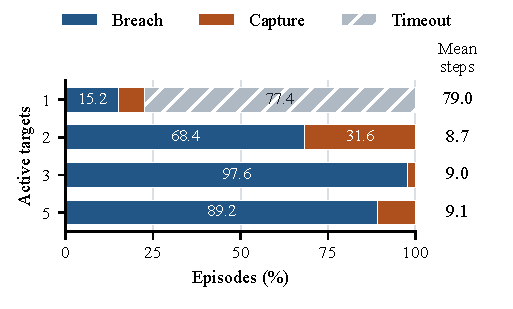
\includegraphics[width=\columnwidth]{paper_figures/multi_target_outcomes_and_duration.pdf}
\caption{}
\label{fig:scaling_diagnostics}
\end{figure}

\subsection{Route use in the $K = 2$ evaluation}
The Attacker won the evaluation in 342 of the 500 episodes. Of those, the Attacker won 128 episodes (37.4\%) at the North target and 214 (62.6\%) at the South target. There were 131 crossings of the North bridge, 128 of the Center bridge and 241 of the South bridge. These counts reflect this run only and do not show the policy would use both targets against other players.

 Fig. \ref{fig:target_choices} shows first bridge entries against the learned Defender and successful target breaches for all four layouts. A breach is counted only if the Attacker reaches a target. First bridge entries can be followed by timeouts or captures.

\begin{figure}[!t]
\centering
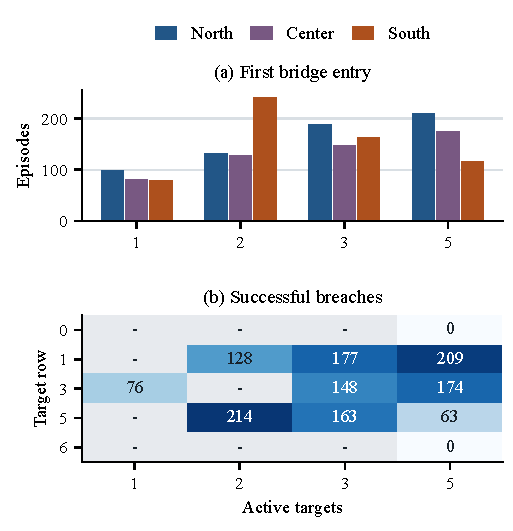
\includegraphics[width=\columnwidth]{paper_figures/multi_target_bridge_and_breach_counts.pdf}
\caption{}
\label{fig:target_choices}
\end{figure}


A separate training audit found that the timeout rate fell from 34.0\% during warm-up to 0.00\% by episode 300. Across 11 saved policy snapshots, the Attacker won 69\% of episodes and the Defender caught it in 30\%. This audit is separate from the 500-episode evaluation behind Tables~\ref{tab:attacker_k_scaling} and~\ref{tab:defender_k_scaling}.

\section{Limitations and Future Work}
Several points limit how far these results can be taken:
\begin{enumerate}
    \item \textbf{Single training run:} The single-target comparisons use 150 paired evaluation seeds per matchup, and the multi-target section uses 500 episodes. All results come from one representative training run per method. Repeating training with several random seeds would show how much the results vary between runs.
    \item \textbf{No direct test of forgetting:} We measure route use and exploitability. We do not test whether an agent loses the ability to use a route, so the link to catastrophic forgetting is only suggested.
    \item \textbf{Archive sampling:} We sample uniformly from the archive, $\mathcal{U}(\mathcal{H})$. In longer training runs this may spend updates on obsolete early policies. Prioritized fictitious play or regret-weighted sampling would be a natural next step.
    \item \textbf{Continuous action spaces:} Moving from discrete grid bottlenecks to continuous navigation would call for ways to compress or cluster the archive.
\end{enumerate}

\section{Conclusion}
In the Three Bridges Arena, we assessed direct self-play and Dual-Archive Co-Evolution. In our primary evaluation, direct self-play favored the North bridge (46.0\% of crossings) over the South (16.1\%). 17.3\% of episodes timed out for the self-play policy. The archive-trained policy showed a higher route entropy and no time outs. Its exploitability was lower (0.140 vs. 0.160) and its security score was better ($-0.187$ vs. $-0.207$), though the win-rate difference was not statistically significant. Based on our results, using the archives helped to keep the use of available routes varied in this case. The study does not evaluate catastrophic forgetting, directly. The results should be verified by more training runs and opponents.

\appendices
\section{Simplified Three-Route Matching Model}
\label{app:matching}
This appendix analyzes a deliberately small model with three Attacker route choices and three Defender guard choices. The Defender's payoff is $+1$ when it guards the route chosen by the Attacker and $-1$ otherwise. With Attacker routes as rows and Defender choices as columns, the payoff matrix is
\begin{equation}
M_D = \begin{bmatrix} +1 & -1 & -1 \\ -1 & +1 & -1 \\ -1 & -1 & +1 \end{bmatrix}.
\end{equation}
There is no pure-strategy equilibrium: when the choices match, the Attacker can switch to an unguarded route; when they differ, the Defender can switch to the Attacker's route. If both players choose uniformly, the Defender's expected payoff against any pure action of the opponent is
\begin{equation}
\mathbb{E}[M_D] = \frac{1}{3}(+1)+\frac{2}{3}(-1)=-\frac{1}{3}.
\end{equation}
The uniform mixtures are minimax strategies for this matching matrix. This result illustrates the value of mixing in the simplified model; it does not establish an equilibrium for the full grid game.

\section*{Acknowledgment}
The authors thank the Department of Mathematics at Sardar Vallabhbhai National Institute of Technology (SVNIT), Surat, for providing computational facilities and academic guidance throughout this work.

\begin{thebibliography}{3}
\bibitem{cliff1995tracking} D. Cliff and G. F. Miller, ``Tracking the Red Queen: Measurements of adaptive progress in co-evolutionary simulations,'' in \textit{Proc. Eur. Conf. Artif. Life (ECAL)}, 1995, pp. 200--218.
\bibitem{ng1999policy} A. Y. Ng, D. Harada, and S. Russell, ``Policy invariance under reward transformations: Theory and application to reward shaping,'' in \textit{Proc. Int. Conf. Mach. Learn. (ICML)}, 1999, pp. 278--287.
\bibitem{schulman2017proximal} J. Schulman, F. Wolski, P. Dhariwal, A. Radford, and O. Klimov, ``Proximal policy optimization algorithms,'' \textit{arXiv preprint arXiv:1707.06347}, 2017.
\end{thebibliography}

\end{document}
